\chapter{Introducción}
\label{ch:introduccion}

El Sol por excelencia es la fuente de energía electromagnética mas potente y abundante en nuestro sistema planetario. El sol por si solo representa mas del 98\% de mas del Sistema Solar, la distancia del Sol a la Tierra es aproximadamente de 150 millones de kilómetros, su luz demora mas de 8 minutos en alcanzar nuestro planeta y además produce 760.000 veces la cantidad de energía consumida en todo el planeta en un año. Tan solo una pequeña porción de toda la energía que esta estrella emite al espacio es recibida por nuestro planeta y aun mas solo una pequeña porción de la energía que llega es aprovechada de manera efectiva. La energía que recibimos del sol es causante de la mayoría de las condiciones climáticas que posee el planeta tierra y que permiten la existencia de la vida como la apreciamos diariamente.\\

\begin{figure}[h!]
        \centering
        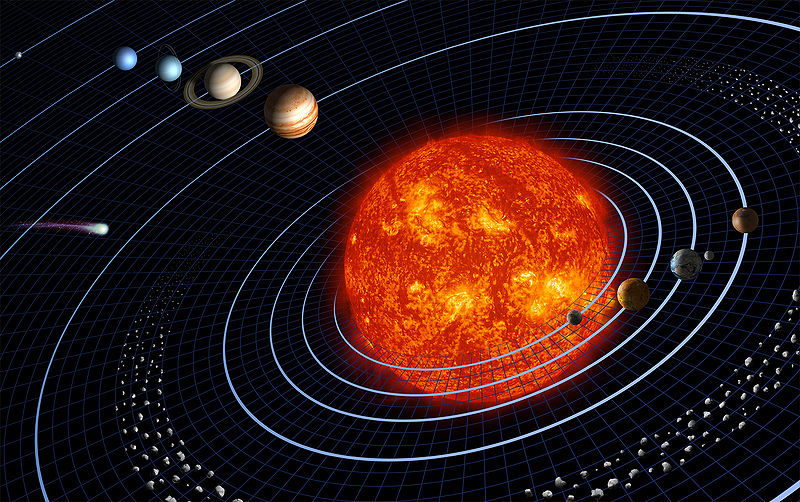
\includegraphics[scale=0.4]{images/solarSis}
        \caption{\tiny Esquema planta fotovoltaica Subsole 307,2 kWp(STC) a la red eléctrica EMELAT - Región de Atacama}
\end{figure}

El trabajo que se presentado a continuación tiene por objetivo desarrollar un sistema informático, que compuesto del software y los instrumentos de precisión adecuados permita exponer a la comunidad información respecto de la producción de energía fotovoltaica de Latinoamérica y el Caribe.\\ 

Fundación Chile es una fundación de carácter privado que se dedica a la creación de valor que aporten al desarrollo del país, dentro de sus áreas de desarrollo cuanta con un área de Energía y cambio climático que a su vez pose un área de Energía Solar. Dentro del área de Energía Solar se encuentran en ejecución, encargado por el banco Interamericano de desarrollo, un proyecto para la creación de una red solar para Latinoamérica y el Caribe(RedSolLac\cite{redSolLac:1}. El objetivo de esta red es generar a corto y mediano plazo una red de coordinación en la región que sea referente en temas de energía solar y que potencie el desarrollo, la investigación y la utilización de la energía solar.\\
 
Como una primera etapa del desarrollo de esta comunidad se encuentra la integración de estaciones de medición instaladas y por instalar en diferentes regiones de chile las cuales pasaran a forma parte de la constitución de una base de datos de radiación de energía solar. Estos datos deben estar disponible a toda la comunidad de manera abierta para aportar en el desarrollo de estas energías.\\

Durante el desarrollo de esta memoria se pretende implementar dos estaciones de medición y desarrollar un software que permita difundir los datos capturados así como herramientas que ayuden en la toma de decisiones respecto de la instalación de equipos productores de energía solar a todo nivel de actividad. En los primero capítulos se abarcaran los alcances de esta memoria y temas introductorios a la energía solar mientras que en los siguientes capítulos describiré de manera de tallada las herramientas desarrolladas y el proceso de implementación, finalmente expondré una fase de captura de datos y prueba del sistema.
